\documentclass[a4paper,12pt]{article}
\usepackage{graphicx}
\usepackage{graphicx}
\usepackage{amssymb}
\usepackage{pifont}
\usepackage{listings}
\usepackage{caption}
\usepackage{subcaption}
\usepackage[english,swedish]{babel}
\usepackage[utf8]{inputenc}
\usepackage[T1]{fontenc}
\newcommand{\cmark}{\ding{51}}%
\newcommand{\xmark}{\ding{55}}%
\lstset{language=c++,
        numberstyle=\footnotesize,
        basicstyle=\ttfamily\footnotesize,
        breaklines=true
    }


\selectlanguage{swedish}
\title{Interactive Solar System}
\author{Gustav Svensk, Johan Jönsson, \\
    Nora Björklund, Christopher Hallberg}
\date{\today}

\begin{document}
\maketitle
\selectlanguage{english}
\tableofcontents
\newpage
\section{Introduction}
% Lista will do och might do
Our finished program is an interactive solar system that follows a subset of 
the laws of physics. The player can move around in the system and configure
initial state of the system.

\subsection{Will Do}
Features that were mandatory are listed in the table below. The check mark
indicates that the feature is implemented.
\begin{center}
        \begin{tabular}{|l|c|}
                \hline
                \textbf{Feature} & \cmark/\xmark \\
                \hline
                Bodies with physical properties & \cmark \\
                Newtonian physics & \cmark \\
                Configurable initial state & \cmark \\
                Collision handling & \cmark \\
                Movable camera & \cmark \\
                Light source(s) & \cmark \\
                Spacebox (skybox but in SPACE!) & \cmark \\
                Asteroid belt & \cmark \\
                Controllable spaceship & \cmark \\
                \hline

        \end{tabular}
\end{center}

\subsection{Might Do}
Feature that were optional are listed in the table below. The check mark
indicates that the feature is implemented.

\begin{center}
        \begin{tabular}[h]{|l|c|}
                \hline
                \textbf{Feature} & \cmark/\xmark \\
                \hline
                Random initial state & \cmark \\
                Relativistic physics (special) & \xmark \\
                Drawing optimized for frustum & \cmark \\
                No sound (because SPACE) & \cmark \\
                Landing on selected bodies (sound?) & \xmark \\
                Build our solar system & \cmark \\
                Trans-neptunian objects (Pluto?, Death star?) & \xmark \\
                Aliens & \xmark \\
                \hline
        \end{tabular}
\end{center}

\section{How To Use}
This section describes how to install and run the program.
\subsection{Setup}
% Hur man kompilerar allt, med soil och allt sånt.
In order to properly compile the source code you first need to compile the SOIL
library included with the source code. To compile SOIL go to
\emph{src/soil/src} and type ``make''. This will compile ``libSOIL.a'' and
place it in the \emph{soil/lib} directory. After you have compiled the SOIL
library you can compile the program normally, return to the root directory of
the program and type make. This will compile all object files needed for the
program and place them in \emph{bin/}, then all the object files will be linked
together to create the executable ``test''.

\subsection{Usage}
The settings for the initial state can be seen in the table below.
\begin{center}
        \begin{tabular}{| l | p{9cm} |}
                \hline
                \textbf{Flag} & \textbf{Action} \\
                \hline
                -h & Display a help message \\
                -s & Creates a sun \\
                -p $np$ & Creates $np$ planets \\
                -r $radius$ & Set the maximum distance from the origin in which
                planets can be created to $radius$\\
                -m $mass$ & Set the maximum mass of the planets to $mass$\\
                -n $mass$ & Set the maximum mass of the sun to $mass + 1E10$ \\
-v $vel$ & Set the maximum initial velocity of the planets to $vel$ \\
                -a $na$ & Create an asteroid belt with $na$ asteroids \\
                \hline
        \end{tabular}
\end{center}
% Hur man startar programmet, inställningar och hur man styr

In the game the ``wasd'' buttons and the mouse are used for navigation.
Other keys can be seen in the table below.
\begin{center}
        \begin{tabular}{|c|l|}
                \hline
                \textbf{Key} & \textbf{Action} \\
                \hline
                p & Save a screenshot to ``space.bmp'' \\
                g & Toggle the locking of keyboard and mouse \\
                left arrow & Decrease simulation step (slower, but more accurate simulation) \\
                right arrow & Increase simulation step (faster, but less accurate simulation) \\
                up arrow & Increase ship speed \\
                down arrow & Decrease ship speed \\
                \hline
        \end{tabular}
\end{center}

\section{Implementation}
This section describes the implementation of the main parts of the program. 
\subsection{Overview}
% UML karta
This project was written in C++ (C++11) using standard C++ libraries (such as
math.h), SDL, OpenGL and SOIL (Simple OpenGL Image Library). We also utilized the libraries created
by Ingemar Ragnemalm for this course (ie. GL\_utilities.h, loadobj.h, LoadTGA.h
and VectorUtils3.h).
\subsection{Celestial Bodies}
% Kanske mer i ordets rätta bemärkelse snarare än structen Cel_bodies?. dvs asteroider.
% Behövs troligtvis inte subsubsections
The celestial bodies are the objects that are affected by gravity in our system
i.e the planets and the sun. They are all subclasses of the class object. The
planets are of the class body which inherits from object. Body's attributes and
functions can be seen in figure XX. The sun is very similar to the planets
except that it also emits sun light. The sun therefore is a subclass that
inherits from body. 

For optimization reasons there is a method for removing objects further away
from the origin than 400 length units.

\subsubsection{Asteroids}
The asteroids are objects that are not gravitationally bound in the system. In 
order to render lots of asteroids on the screen we could not use the
gravitational calculations to update the positions of all the asteroids. Instead
we decided to make the asteroids follow a circular orbit some great distance
from the origin, this way we still get a somewhat realistic result and we save a
lot of computational power. This way of treating asteroids differently from
other celestial objects also, unfortunately, means that we cannot use our
methods for frustum culling. Thus all asteroids in the system are rendered at
all times.

\subsection{Spacebox \& Ship (Cat?)}
The drawing of the spacebox and the ship is handled specially in the shaders.
This is because the spacebox is always drawn around the camera and is therefore
only dependent of the rotation part of the camera matrix and the lighting does
not affect the spacebox. The ship is always drawn in front of the camera and is
not dependent on the camera matrix. To let the shaders know that the object
drawn is a spacebox or a ship a uniform int is sent to the shaders. Examples
can be seen in listings \ref{lst:ship} and \ref{lst:vert}.

\begin{lstlisting}[caption={Draw spaceship}, label={lst:ship}]
glUniform1i(glGetUniformLocation(program, "spaceship"), 1);
...
Draw ship here
...
glUniform1i(glGetUniformLocation(program, "spaceship"), 0);
\end{lstlisting}

\begin{lstlisting}[caption={Vertex shader}, label={lst:vert}]
if(spacebox == 0 && spaceship == 0){
    gl_Position = proj_matrix * cam_matrix * mdl_matrix * vec4(in_position, 1.0);
} else if(spaceship == 1 && spacebox == 0)
    gl_Position = proj_matrix * mdl_matrix * vec4(in_position, 1.0);
else {
    gl_Position = proj_matrix * mat4(mat3(cam_matrix)) * mdl_matrix * vec4(in_position, 1.0);
} 
\end{lstlisting}

\subsection{Physics}
The program implements Newtonian gravity in order to obtain the acceleration of
each body and then integrates this acceleration into velocity and then the
velocity is integrated into position.

Newton's laws of motion tells us that $F=ma \Leftrightarrow a = \frac{F}{m}$.
Newton's theory for gravity tells us that $F_{1,2} = G\frac{m_1m_2}{r}$, where
$F_{1,2}$ is the gravitational force generated by body 1 acting on body 2 and
$G$ is the gravitational constant. Now we also now that each force has an equal
and opposite force (Newton's third law), this tells us that $F_{1,2} =
F_{2,1}$, since they are both scalar values and therefore contains no notion of
direction.

In order to properly use these relations we need to add the concept of
direction, this is easy to do and the result is.
\[
\bar{a} = \frac{\bar{F}}{m}
\]
\[
\bar{F_{1,2}} = G\frac{m_1m_2}{|\bar{r}|^2}\hat{r} \, , \, \hat{r} = \frac{\bar{r_1} - \bar{r_2}}{|\bar{r_1} - \bar{r_2}|}
\]
And now we can calculate the resulting force on body $i$, with $n$ bodies in total
\[
\bar{F_i} = G m_i\sum_{k=1}^n \frac{m_k}{|\bar{r_i} - \bar{r_k}|^3}\left( \bar{r_i} - \bar{r_k} \right)
\]
This then gives us the acceleration on the body $i$
\[
\bar{a_i} = G \sum_{k=1}^n \frac{m_k}{|\bar{r_i} - \bar{r_k}|^3}\left( \bar{r_i} - \bar{r_k} \right)
\]

Using these values and the initial positions and velocities of each planet we
are now ready to integrate the velocities and positions. For this we use the
Runge-Kutta-4 numerical method for solving first order differential equations.
Now, acceleration is the first time-derivative of velocity ($a=\ddot{p} =
\dot{v}$) which in turn is the first time-derivative of position ($v=\dot{p}$).
So we actually have to do two RK4 solutions, one to obtain the velocity and
another to obtain the position.

Below I give the general RK4-method
\[
\dot{y}=f(t,y),\,y(t_0)=y_0
\]
\[
y_{n+1} = y_n + \frac{1}{6}h\left( k_1 + 2k_2 + 2k_3 + k_4\right)
\]
\[
t_{n+1} = t_n +h
\]
\[
k_1 = f(t_n,y_n)
\]
\[
k_2 = f(t_n + \frac{1}{2}h,y_n + \frac{h}{2}k_1)
\]
\[
k_3 = f(t_n + \frac{1}{2}h,y_n + \frac{h}{2}k_2)
\]
\[
k_4 = f(t_n + h,y_n + hk_3)
\]
Where $h$ is our time-step (our program begins with $h = 0.002$), the numerical
error of this method is of the order $\mathcal{O}(h^5)$

\subsection{Collision}
The collision functionality of celestial bodies is implemented by two methods
in the system class, one for collision detection and one for collision
handling. When the method for detection is called, a vector
between the centres of the two bodies is calculated. Then the squared distance
of this vector is compared with the squared distance of the radii. If the
squared distance of the difference between the two centres is smaller or equal
to the squared distance of the radii the bodies collide.
The simplicity of the detection is due to the spherical properties of the
celestial bodies.

The method for handling collisions is called
every time the system uses the update method. Each time the method is called it
loops through the linked list with the celestial bodies, comparing all bodies
with each other. For each iteration detection method is called, if bodies
do not collide nothing happens and the comparison continues. If, however, two
bodies collide new properties are calculated based upon perfectly-plastic
collisions. The new mass will be the combined masses of the colliding bodies,
the new radius will be the cube root of the original radii cubes added together
and the new velocity is calculated from the notion of preservation of momentum.
Then the original masses are compared and the body with the smallest mass is
deleted from the linked list while the one with the bigger mass will be updated
with the newly calculated properties.

This is a brute force approach and could be optimized, but it works well for a
reasonable amount of bodies. Furthermore, the performance is limited mainly by
the physics calculations. Possible optimizations could be not to call the
collision handling at a lower frequency than the rest of the updates since it
would not make any visible difference for the human eye. Another possible way
could be to divide the space into different sectors and only compare bodies
within the sectors. 

The collision handling only affects the bodies in the linked list of suns and
planets. The asteroids and ship are not effected by this functionality.

\subsection{Camera \& Frustum}
The standard frustum is 300 length units, but can be changed in test.cpp if
needed. Frustum culling is used to avoid drawing objects outside of the
frustum. Instead of using extraction of planes as suggested in the lectures,
projection of vectors is used. Frustum culling is not used for the top and
bottom planes, the reason for this will be described in further detail in
section \ref{sec:up_prob}.


\section{Problems}
This section discusses the current problems with the program.
\subsection{Up-vector \& Frustum Culling}
\label{sec:up_prob}
The problem with the up-vector is that if the ``look-at vector'' is parallel
with the up-vector, we get a multiplication by zero and  only the background
color is shown. To fix this it is forbidden to look straight up. This is
implemented by checking if the mouse position has y-component that is zero, if
it is so, it is forced to one. With this implementation the up-vector can be
fixed to (0,1,0). 


Another problem which is caused by the fixed up-vector is that the
frustum culling cannot be performed on the top and bottom planes. This is
because the frustum culling uses the up-vector to decide if an object is inside
the frustum or not. The culling assumes an updated up-vector, but since it is
fixed the culling of those planes is not performed.


A more elegant solution to both of these problems is to make the up-vector
follow the camera, but when this was tried the ship navigation became near
impossible.
\subsection{Multiple Suns}
It is possble to implement two suns at the moment but the light from them will
not be correct. This happens because we upload the light from the celestial
bodies list, and in the fragment shader the light will be calculated according
to the latest uploaded light source only and not both of them. To solve this we
need to upload the light as an array and then calculate the light combined. For
the array solution to work the number of suns needs to be limited too since it
is not possible to have a array of undecided length in the fragment shader.
\section{Conclusions}

\section{Screenshots}
Here be screenshots.
\begin{figure}[h!]
        \centering
        \centerline{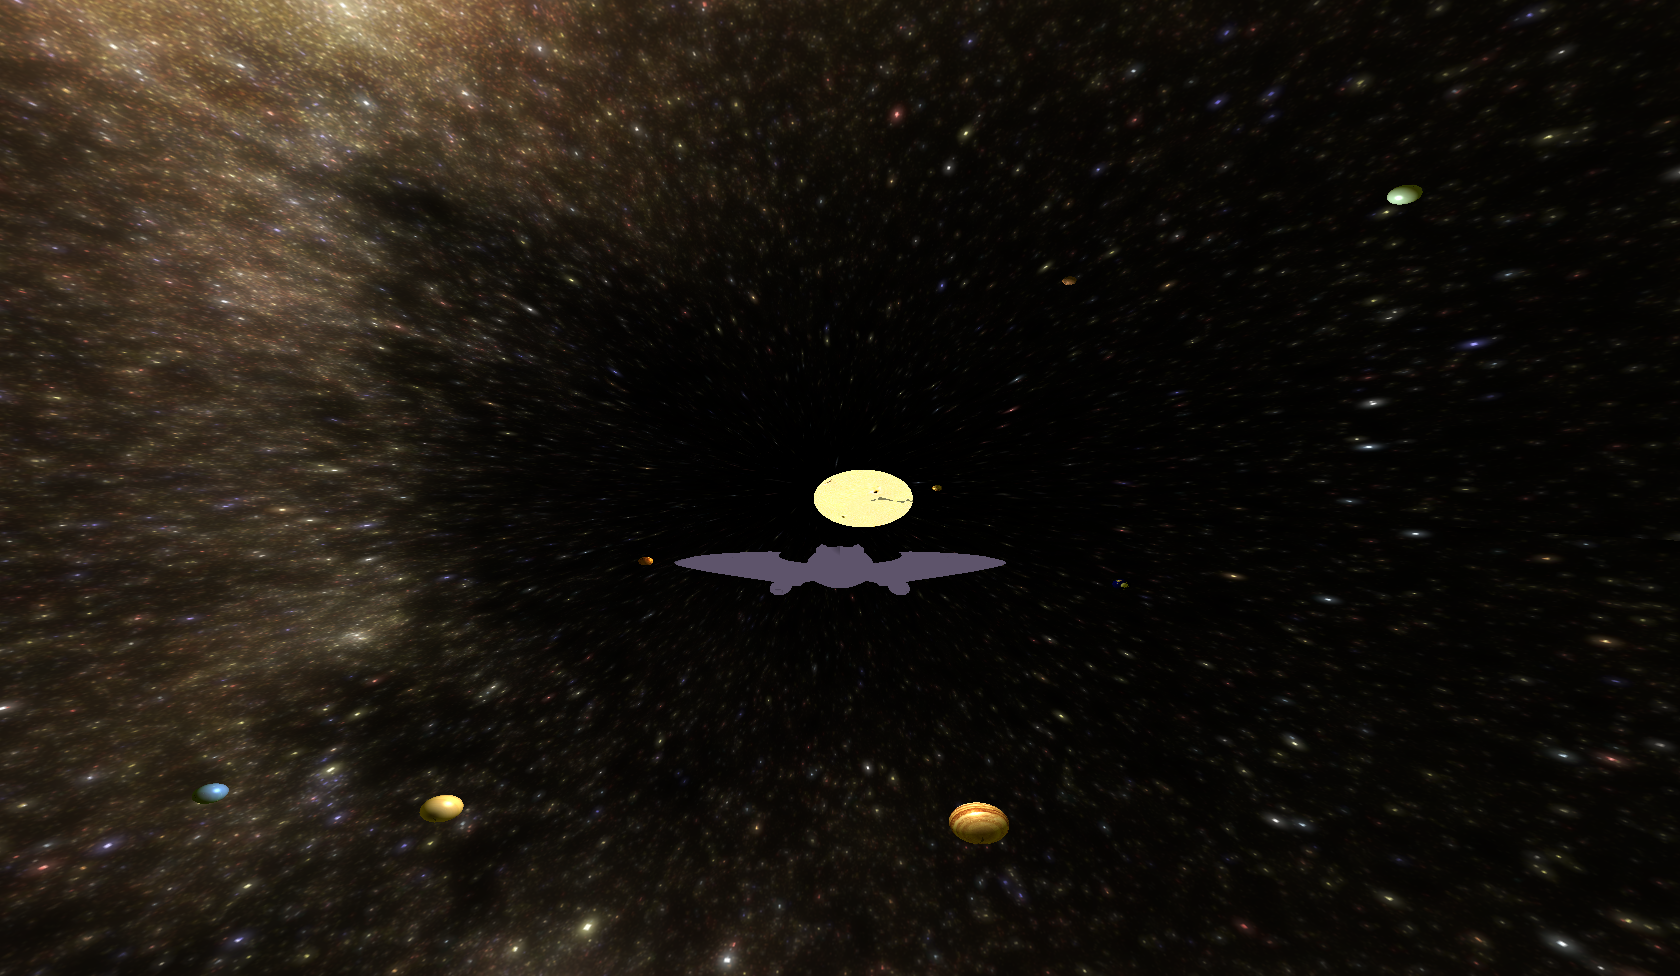
\includegraphics[width=1.2\textwidth]{bild/our.png}}
        \caption{Our solar system}
        \label{fig:our}
\end{figure}
\begin{figure}[h!]
        \centering
        \centerline{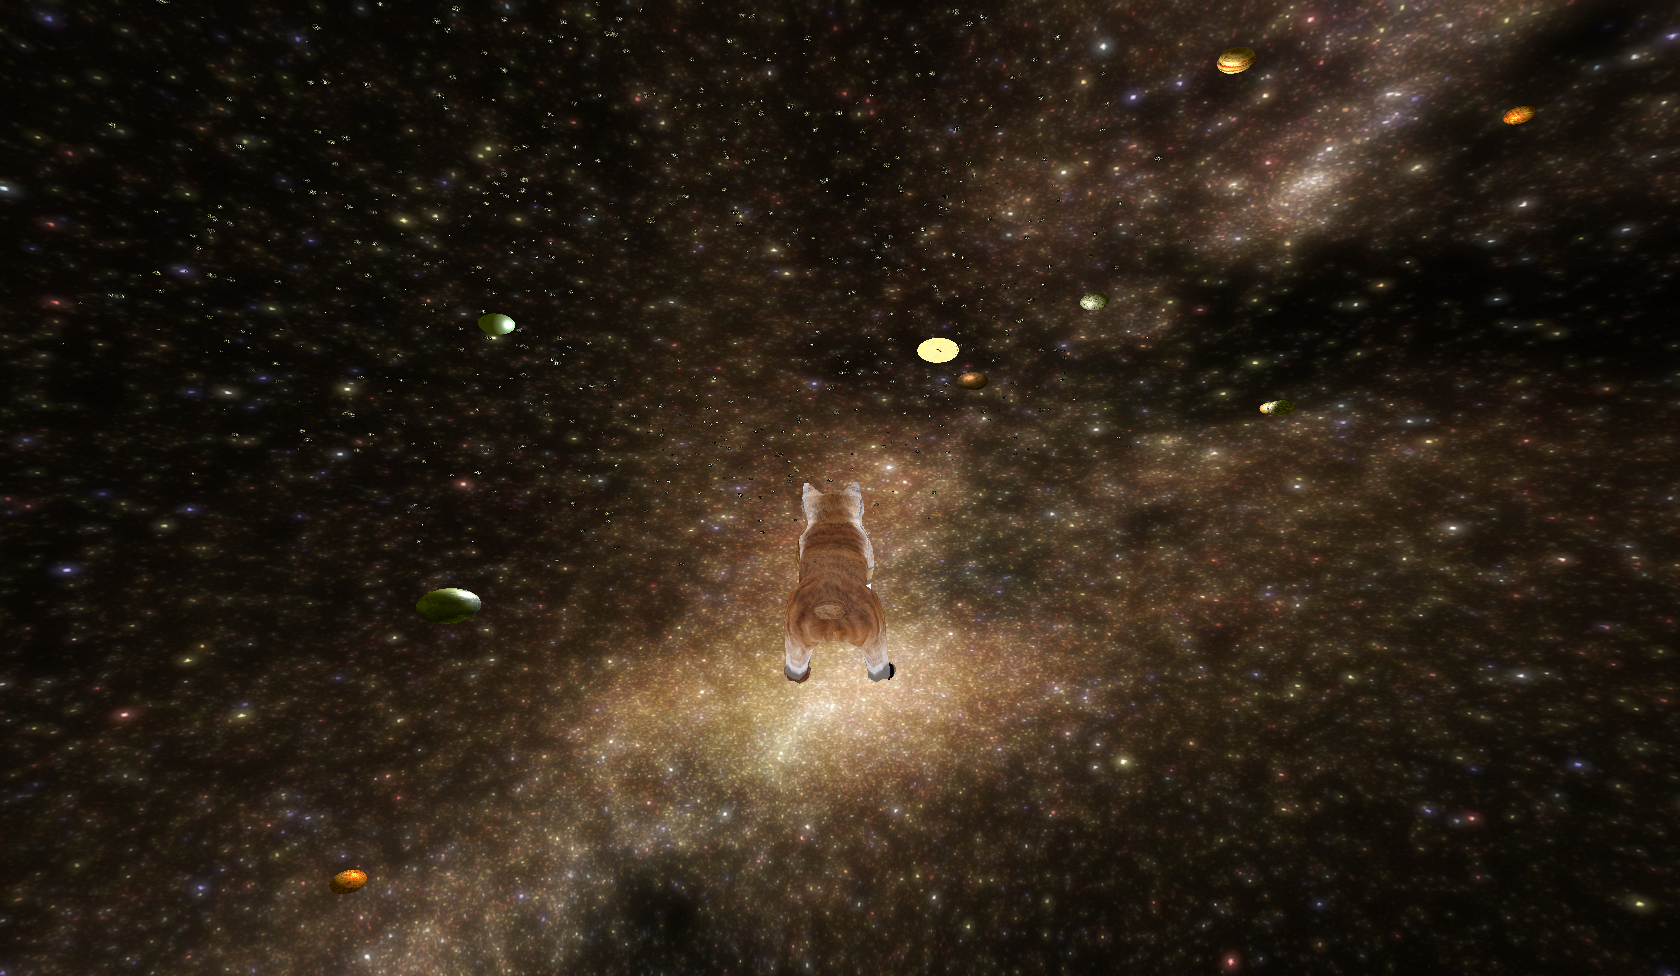
\includegraphics[width=1.2\textwidth]{bild/cat.png}}
        \caption{Catship}
        \label{fig:cat}
\end{figure}
\begin{figure}[h!]
        \centering
        \centerline{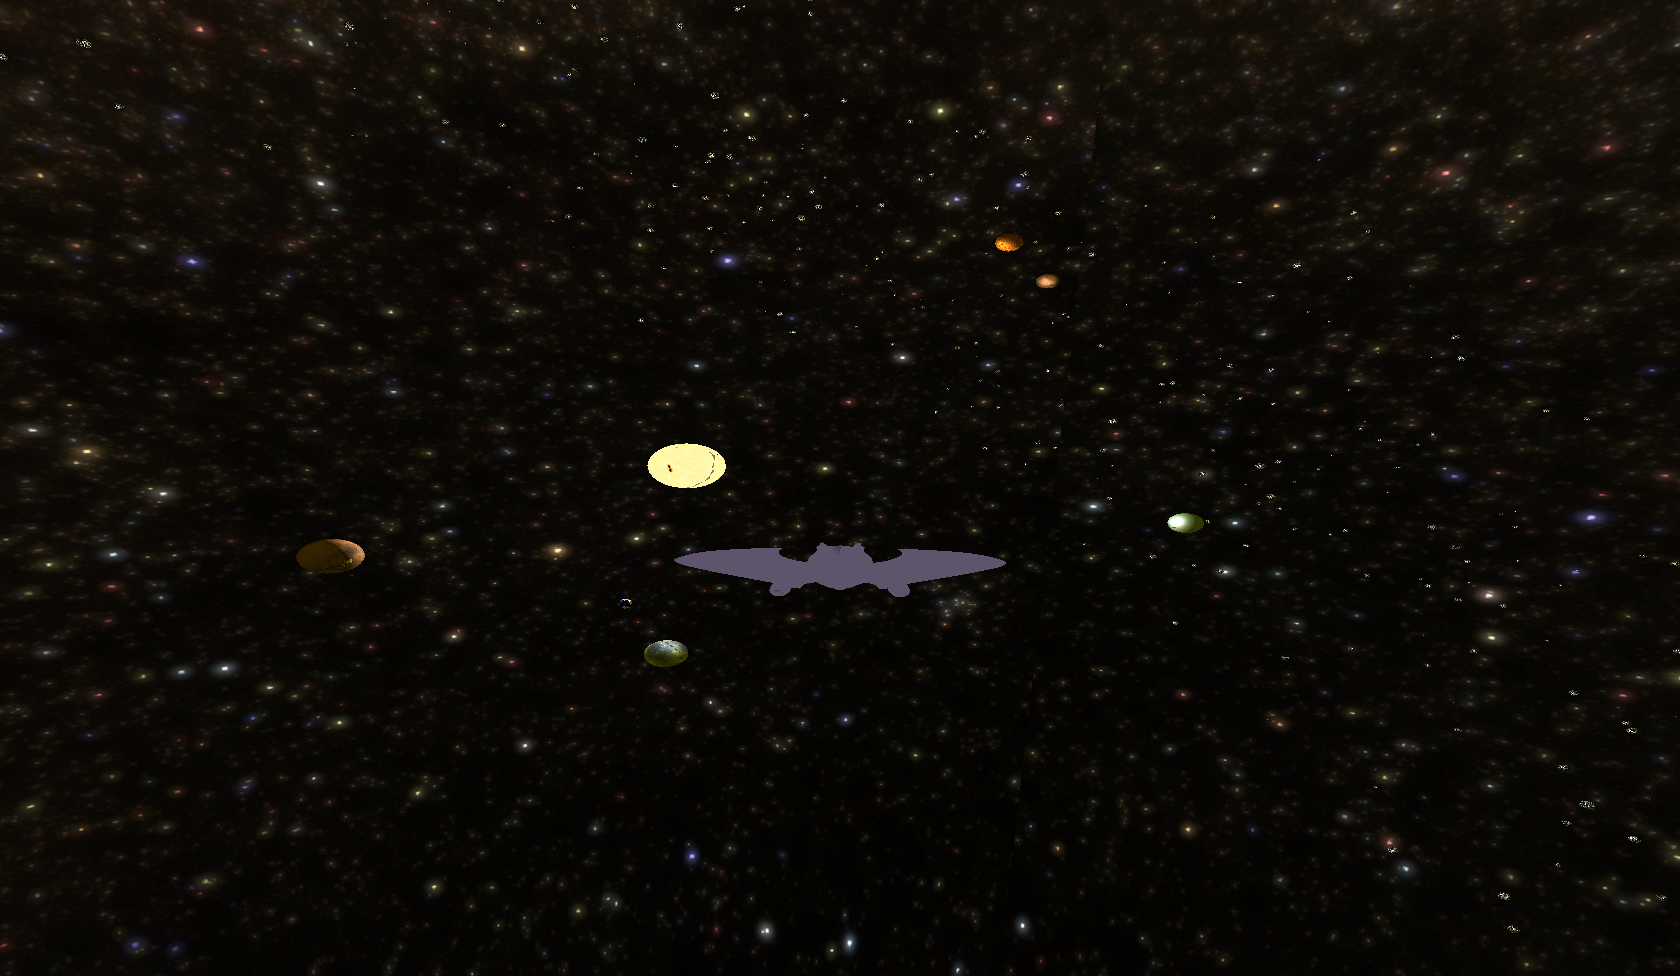
\includegraphics[width=1.2\textwidth]{bild/planets.png}}
        \caption{Planets}
        \label{fig:planets}
\end{figure}
\begin{figure}[h!]
        \centering
        \centerline{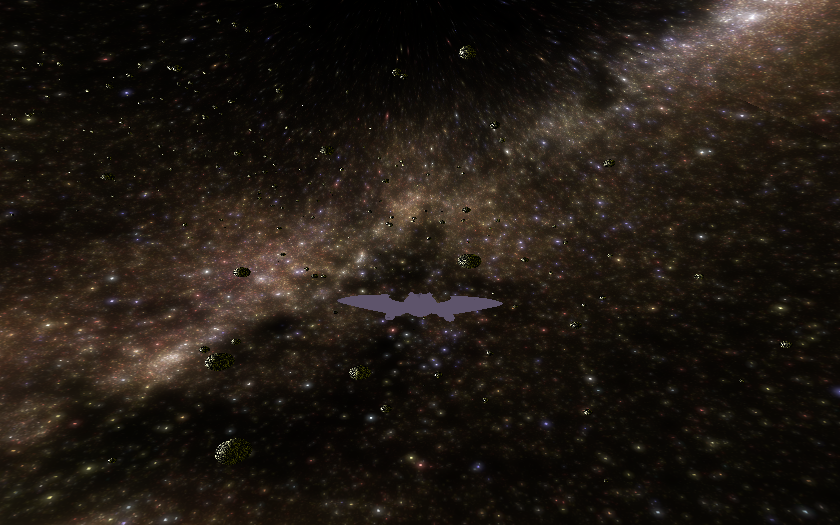
\includegraphics[width=1.2\textwidth]{bild/asteroid.png}}
        \caption{Asteroids}
        \label{fig:asteroids}
\end{figure}
\end{document} 
% Local Variables: %%% mode: latex %%% TeX-master: t %%% End:
